\maketitle

\begin{abstract}
When a Lean proof attempt fails, the pipeline records how: the output was cut off at the token limit, Lean timed out, or Lean reported an error such as an unsolved goal.  The usual practice is to put this information into the next prompt.  We instead give it to the retry policy, which decides which failed theorem gets another attempt and when to stop.  Our testbed is a quantized Goedel-Prover-V2-8B on one RTX 4090, retrying the 40 held-out miniF2F theorems whose first attempt failed.  The scheduling study (S1) was introduced in our earlier workshop paper; we re-audit it here and add three new studies.  In S1, never retrying a theorem whose first attempt timed out saves 10.8\% and 11.3\% of retry tokens in two independent sets of retry seeds, and loses no theorem in any of the 24 draw orderings we replay.  The full rule set also allows at most two retries for theorems whose first attempt was truncated and orders the remaining retries by failure class.  It saves \SchedBOneSavings{} and \SchedBTwoSavings{} in the pre-specified ordering, and medians of \SchedBOneOrderMedian{} and \SchedBTwoOrderMedian{} over the orderings in which it matches uniform retrying's solve count.  It matches that count in only \SchedBOneParity{} and \SchedBTwoParity{} orderings and ends one theorem short in the others.  Caps that ignore the failure class save less or lose more theorems.  Re-timing \AllBranches{} recovery attempts (S2) shows that prompt prefill takes \PrefillServingShare{} of serving time, while generations that hit the output cap take \TruncatedTotalShare{} of measured prefill, decode and Lean time and never reach Lean.  Splitting a fixed token budget into more, shorter attempts (S3) shows no detectable gain on held-out theorems and spends more tokens per theorem.  In a prospective test on three new seed sets (S4), an 8,192-token cap on first-attempt-truncated theorems solved the same theorems as the 12,288-token baseline and saved \CrCapEnergyPooled{} of measured GPU energy (post hoc \ci{} \CrCapEnergyPooledCI{}).
\end{abstract}

\section{Introduction}

A theorem-proving agent whose proof fails must decide what to do next.  It can retry, attempt a repair, or drop the theorem and spend its budget elsewhere, and these decisions set how much compute it spends on theorems it cannot yet prove.  A retry that decodes all the way to the 12,288-token output limit, or one that waits 180 seconds for a Lean timeout, costs far more than an average attempt and may still prove nothing.  Counting attempts, or the token budget a policy is allowed, hides these differences.

The usual approach shows the model the error message or its failed proof and asks it to try again.  In our earlier paper \citep{reddy2026scheduling}, twelve retry prompts that added hints keyed to the failure class, without showing the failed proof, did not reliably beat plain resampling.  In a companion paper \citep{reddy2026sticky}, showing the model its rejected proof mostly led it to carry over the lines tied to that proof's first error.  The failure report can also be used by the controller instead of the model.  A timeout gives the model little to work with, yet it may be a good sign that another attempt will be expensive and unlikely to succeed.

We test this idea on a small Lean workload and record what each policy actually spends.  Table~\ref{tab:studies} lists the four studies.  S1 was introduced in our earlier paper; here we recompute it from the recorded draws and add controls that cap retries without using the failure class.  S2--S4 are new; S2 re-times attempts generated for the companion paper.  The main findings are as follows.
\begin{itemize}[leftmargin=*,itemsep=1pt,topsep=2pt]
  \item Never retrying after a Lean timeout is the most reliable rule.  It saves about 11\% of retry tokens and loses no theorem in any of the 24 draw orderings.
  \item Limiting retries after a truncated first attempt saves more, because those retries are expensive rather than because they rarely succeed.  On held-out theorems, truncated roots are rescued per token somewhat less often than the average root but about \CrTruncRhoGap{} as often as the development estimate, and the limit loses a theorem in some orderings.  Caps that ignore the failure class do worse.
  \item In this serving stack prompt prefill is cheap, under 1\% of serving time.  Generations that run to the output cap take \TruncatedTotalShare{} of measured time and never reach Lean.
  \item On held-out theorems, splitting a fixed budget into more, shorter attempts showed no detectable gain and spent more tokens per theorem.  On development theorems two shorter attempts did better, so the yield question remains open.
  \item An 8,192-token cap on first-attempt-truncated theorems kept every solved theorem in three new seed blocks and reduced GPU energy by \CapJoulesSavedRange{} per block.  Applying the same cap to every theorem saved more tokens but lost one theorem.
\end{itemize}

\begin{table}[t]
\caption{The four studies.  Apart from S1's small transfer cohorts and the four-slot check in S2, all four use Goedel-Prover-V2-8B on the same single-slot serving stack and the same 83 failed first attempts.  S3's Long arm reuses S2's arm-A attempts; no analysis pools draws across studies.  \emph{Roots} are theorems whose first attempt failed.}
\label{tab:studies}
\centering\small
\begin{tabularx}{\linewidth}{@{}l>{\raggedright\arraybackslash}X>{\raggedright\arraybackslash}Xl>{\raggedright\arraybackslash}X@{}}
\toprule
Study & Question & Data & Status & Main endpoint \\
\midrule
S1 & Which failed theorem gets the next retry? & 40 held-out roots, 4 recorded retries each, 2 seed blocks & Inherited, re-audited & Retry tokens spent to reach uniform's solve count \\
S2 & Where does serving time go? & \AllBranches{} recovery attempts on all 83 roots & New analysis & Share of measured time in prefill, decode and Lean \\
S3 & Do more, shorter attempts help at a fixed budget? & 40 held-out roots, 1 seed block & New; Long from S2 & Paired verification rate against one long attempt \\
S4 & Does an 8,192-token cap on truncated roots lose proofs? & 40 held-out roots, 3 new seed blocks & New, prospective & Paired verified count; tokens and GPU energy \\
\bottomrule
\end{tabularx}
\end{table}

\paragraph{Related work.}
Formal provers spend test-time compute on whole-proof sampling, retrieval, feedback-driven repair and search \citep{first2023baldur,yang2023leandojo,thakur2024copra,lin2025goedel,ren2025deepseekproverv2,wang2025kimina,ma2026oprover}.  Repeated sampling works but is expensive \citep{brown2024monkeys}, and several papers allocate test-time compute adaptively \citep{snell2024scaling,alomrani2025budget,zuo2025bandit,wang2025rollout,damani2025think,zhai2026adaptive}.  The closest work is by \citet{rognvaldsson2026cost}, who learn a cost-quality router for an agentic Lean prover.  We do not train a router.  We evaluate a few hand-written rules driven by the failure class of the first attempt, using exact replay, and we measure cost by serving phase and, in S4, by GPU energy.  LLM serving distinguishes a parallel prompt-prefill phase from a sequential decode phase \citep{agrawal2023sarathi,kwon2023vllm}, and we use the same split to locate the cost.

\section{Setup}
\label{sec:setup}

\paragraph{Prover and verifier.}
Unless stated otherwise, runs use a Q4\_K\_M quantization of Goedel-Prover-V2-8B \citep{lin2025goedel} served by a pinned llama.cpp build \citep{gerganov2023llamacpp} on one RTX 4090, with one request slot, no prompt cache, no continuous batching, a 32,768-token context, temperature 0.7, top-$p$ 0.95, top-$k$ 40, min-$p$ 0.05, and at most 12,288 output tokens.  Proofs are checked one at a time in a pinned \lean{}/mathlib environment with a 180-second timeout \citep{moura2021lean,mathlib2020}.

\paragraph{Theorems and roots.}
We use \MiniFTwoFUsed{} miniF2F-test statements \citep{zheng2021minif2f}.  These are the full \MiniFTwoFTest{} minus \MiniFTwoFExcluded{} that were inspected while debugging the earlier paper's harness and set aside before any run reported here (Appendix~\ref{app:relationship}).  A first attempt proves \SchedStageOneVerified{} of them, and we call the 83 failed theorems \emph{roots}.  Before any retry was generated, the roots were split, stratified by failure class, into 43 \emph{development} roots for fitting the rules and 40 \emph{held-out} roots for evaluating them.

\paragraph{Failure classes.}
A fixed function of the model response and the Lean output assigns each attempt one class (Appendix~\ref{app:cap-details}).  The 83 roots fall into seven classes: \emph{truncated} (the output hit the token cap, so Lean never ran), \emph{timeout}, \emph{unsolved goals}, \emph{linarith failed}, \emph{unknown identifier}, \emph{simp failed} and \emph{other}.  The classifier has three further classes that no root here falls into.  A root's class is the class of its first attempt.

\paragraph{Draws, seed blocks and orderings.}
A \emph{draw} is one retry of a root.  Its prompt is the theorem statement alone, it uses a fresh seed, and it has no memory of earlier attempts.  A \emph{rescue} is a draw that verifies.  A \emph{seed block} is one set of draws on the 40 held-out roots generated from one range of seeds.  A second seed block re-samples the retries on the same theorems, so it measures sensitivity to sampling noise and says nothing about new theorems; we never pool blocks.  In S1 each root has four recorded draws per block, and a \emph{draw ordering} is a permutation of the four draw positions, applied to every root at once, giving $4!=24$ orderings.  The \emph{primary} ordering is the order in which the draws were generated, which the earlier paper's replay code fixed in advance.  We report all 24.  Block numbers are local to each study.  S1's two blocks are retry draws from the earlier paper, S2's held-out blocks~1 and~2 and its development cohort are the companion study's recovery attempts, and S4's three blocks are new.  The studies share theorems but not draws, except that S3's Long arm reuses S2's arm-A attempts.

\paragraph{Policies.}
\emph{Uniform} retrying is round-robin: one draw for every unsolved root, then a second, up to four.  The \emph{frozen rules} change three things.
\begin{enumerate}[leftmargin=*,itemsep=1pt,topsep=2pt]
  \item Never retry a root whose first attempt timed out.
  \item Retry at most twice any root whose first attempt was truncated.
  \item Within each round, serve roots in a fixed class order.
\end{enumerate}
Rule~3 ranks classes by development rescues per completion token.  Each class's rescue rate is first shrunk toward the development average (\CrGlobalRate{}) by eight pseudo-attempts, which is why \emph{simp failed} (0 of 4 rescues) ranks above \emph{truncated} (3 of 68); Appendix Table~\ref{tab:class-formula} lists every value.  Rule~3 only reorders a round and never withholds a retry.  The rules were fit on development roots only and were not changed afterwards.

\paragraph{Replay and endpoints.}
All S1 policies consume the same recorded draws and differ only in which draws they use and in what order.  The main endpoint is the number of retry tokens a policy spends before it reaches uniform's final solve count.  A policy reaches \emph{parity} in an ordering if it gets there at all.  A deployed controller does not know uniform's final count, so we also report total spend when a policy runs out of eligible draws, which we call \emph{exhaustion}.  Uncertainty comes from 10,000 theorem-level bootstrap resamples on the primary ordering and from the spread over all 24 orderings.

\paragraph{What runs where.}
The S1 replays use the earlier paper's simulator unchanged, and our scripts reproduce its published ablation values for the four rule variants exactly.  Our harness, \path{src/agent_loop.py}, replays two fixed per-root plans from S2 on held-out block~1 (one regenerate call, or one repair call, per root) and the two S3 split plans on the held-out roots, and checks six invariants covering plan conformance, budget, stopping on verification, accounting, determinism and non-adaptivity.  A fault-injection test confirms that its monitor catches \HarnessDetected{} injected faults (Appendix Table~\ref{tab:faults}).  The harness does not run the S1 scheduler.

\section{S1: scheduling retries by failure class}
\label{sec:scheduler}

\begin{table}[t]
\caption{S1 on the 40 held-out roots.  \emph{Saving}: reduction in retry tokens needed to reach uniform's final solve count, primary ordering.  \emph{Parity}: orderings, of 24, in which the rules reach that count; in the others they end one theorem short.  \emph{Median}: median saving over the parity orderings only.  \emph{Exhaustion}: reduction in total spend when each policy runs out of draws, primary ordering, where both end on the same count.}
\label{tab:scheduler-main}
\centering\small
\begin{tabular}{lrrrrrrr}
\toprule
Block & Solves & Uniform tok. & Rules tok. & Saving & Parity & Median & Exhaustion \\
\midrule
1 & \SchedBOneSolves{}/40 & \SchedBOneTokensUniform{} & \SchedBOneTokensRules{} & \SchedBOneSavings{} & \SchedBOneParity{} & \SchedBOneOrderMedian{} & \SchedBOneExhaustSavings{} \\
2 & \SchedBTwoSolves{}/40 & \SchedBTwoTokensUniform{} & \SchedBTwoTokensRules{} & \SchedBTwoSavings{} & \SchedBTwoParity{} & \SchedBTwoOrderMedian{} & \SchedBTwoExhaustSavings{} \\
\bottomrule
\end{tabular}
\end{table}

\paragraph{Main result.}
In the primary ordering of block~1, both policies solve \SchedBOneSolves{} of the 40 held-out roots.  The rules reach that count with \SchedBOneTokensRules{} retry tokens, against \SchedBOneTokensUniform{} for uniform (Table~\ref{tab:scheduler-main}).  In block~2 both solve \SchedBTwoSolves{}, with \SchedBTwoTokensRules{} tokens against \SchedBTwoTokensUniform{}.  Generation and verification time, summed over the recorded attempts, falls by \SchedTimeBOne{} and \SchedTimeBTwo{}.  In the primary ordering both policies also end on the same solve count when run to exhaustion, and the rules spend \SchedBOneExhaustSavings{} and \SchedBTwoExhaustSavings{} fewer tokens, so there the saving does not rely on knowing when to stop.  In the orderings without parity, the rules end one theorem short even at exhaustion.  Including the shared first pass over 202 theorems, the pipeline uses \SchedPipelineOneSavings{} and \SchedPipelineTwoSavings{} fewer completion tokens and makes \SchedPipelineOneCallsAvoided{} and \SchedPipelineTwoCallsAvoided{} fewer model calls (Appendix Table~\ref{tab:pipeline}).

For block~1 the primary ordering is a favorable one.  Across the 24 orderings the rules reach parity in \SchedBOneParity{}, with a median saving of \SchedBOneOrderMedian{} over those orderings.  A theorem-level bootstrap of the primary-ordering saving gives \CrBOneBoot{} (median and 95\% interval), an interval that includes zero.  Block~2 holds up better, with parity in \SchedBTwoParity{} orderings, a median of \SchedBTwoOrderMedian{} and a bootstrap of \CrBTwoBoot{}.  Figure~\ref{fig:scheduler} shows the block-1 curves.

\begin{figure}[t]
\centering
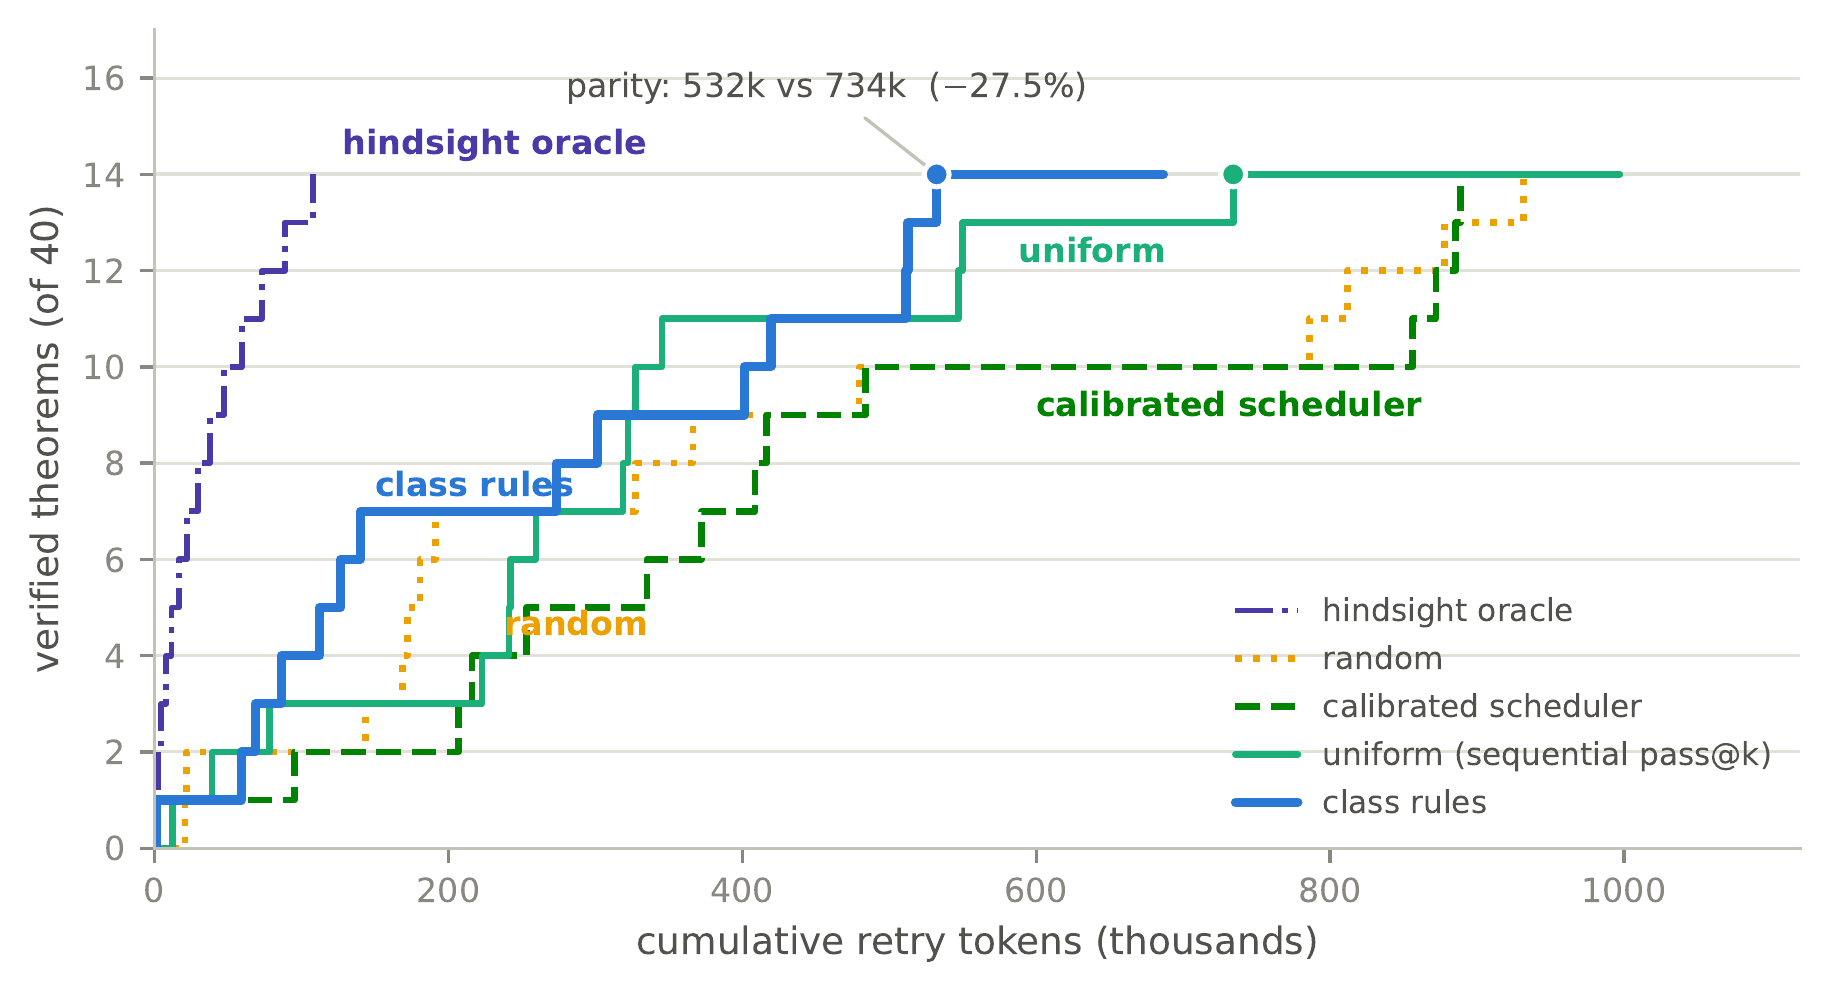
\includegraphics[width=.82\linewidth]{figures/scheduler_budget.png}
\caption{Held-out roots solved as the retry-token budget grows, block~1, primary ordering.  \emph{Class rules} is the frozen policy.  The calibrated scheduler, random order and hindsight oracle are replay comparators defined in Appendix~\ref{app:scheduler-details}.}
\label{fig:scheduler}
\end{figure}

\begin{table}[t]
\caption{Contribution of each rule, and of the failure class.  Each variant replays the same draws in all 24 orderings.  \emph{Parity}: orderings that reach uniform's solve count.  \emph{Loss}: largest shortfall, in theorems, over the 24 orderings.  \emph{Saving}: median over the 24 orderings of the token saving at exhaustion, relative to uniform's full spend.  The lower rows ignore the failure class, apart from the timeout rule in the last row.  Class order affects only the sequence in which draws are spent, so the full rules and the two coarse clauses spend the same at exhaustion.}
\label{tab:controls}
\centering\small
\begin{tabular}{lrrrrrr}
\toprule
& \multicolumn{3}{c}{Block 1} & \multicolumn{3}{c}{Block 2} \\
\cmidrule(lr){2-4}\cmidrule(lr){5-7}
Variant & Parity & Loss & Saving & Parity & Loss & Saving \\
\midrule
\inputrows{tables/cr_s1_controls.tex}
\bottomrule
\end{tabular}
\end{table}

\paragraph{Which rules do the work.}
Table~\ref{tab:controls} replays each rule on its own.  The timeout rule alone saves 10.8\% and 11.3\% of tokens at exhaustion, nearly the same as at uniform's solve count, and never loses a theorem.  No timeout root was rescued in either block or in the development set (0 of 12 draws in each set, on three roots per set).  Three roots is a small base, and we would not expect the rule to carry over unchanged to other workloads.  The truncation limit accounts for most of the remaining saving and for all of the ordering risk.  Class order does not help consistently.  Without it, the two limits save \CrBOneCoarsePrimary{} and \CrBTwoCoarsePrimary{} in the primary ordering, against \SchedBOneSavings{} and \SchedBTwoSavings{} for the full rules, and \CrBOneCoarseParityMedian{} and \CrBTwoCoarseParityMedian{} as medians over parity orderings, against \SchedBOneOrderMedian{} and \SchedBTwoOrderMedian{} (Appendix Table~\ref{tab:ablation}).  A calibrated allocator that re-ranks roots as attempts accumulate does worse than the fixed rules: its token saving in the primary ordering is \SchedCalibratedBOne{} in block~1, meaning it spends more than uniform, and \SchedCalibratedBTwo{} in block~2.

\paragraph{Does the class matter, or only the cap?}
The lower rows of Table~\ref{tab:controls} cap retries without using the failure class.  A cap of two retries on every root saves \CrBOneCapTwoExhMedian{} and \CrBTwoCapTwoExhMedian{} but never reaches parity, losing \CrBOneCapTwoMinLoss{}--\CrBOneCapTwoMaxLoss{} theorems in block~1 and \CrBTwoCapTwoMinLoss{}--\CrBTwoCapTwoMaxLoss{} in block~2.  A cap of three loses no more than the rules in block~1 but saves less, and in block~2 it loses up to three theorems where the rules lose at most one.  Skipping timeouts and capping every other root at three saves \CrBOneToCapThreeExhMedian{} and \CrBTwoToCapThreeExhMedian{}, close to the rules in block~1 but less in block~2, and loses up to \CrBTwoToCapThreeMaxLoss{} theorems in block~2.  The failure class therefore picks out roots whose retries can be cut with little loss, which a uniform cap cannot do.

\paragraph{The truncation rule limits cost.}
We motivated rule~2 with the development data, where truncated roots had 3 rescues in 68 draws, or 0.46 rescues per $10^5$ tokens against 1.71 for all development roots.  The held-out roots did not bear this out.  Their truncated roots had \CrBOneTruncRescues{} rescues in \CrBOneTruncAttempts{} draws in block~1 and \CrBTwoTruncRescues{} in \CrBTwoTruncAttempts{} in block~2, or \CrBOneTruncRho{} and \CrBTwoTruncRho{} per $10^5$ tokens against \CrBOneAllRho{} and \CrBTwoAllRho{} for all held-out roots (Appendix Table~\ref{tab:heldout-ledger}).  Per token, a held-out truncated root is rescued somewhat less often than the average held-out root, and the development estimate was about \CrTruncRhoGap{} too low.  A truncated first attempt does predict cost.  In both blocks, \CrBOneTruncPersist{} of draws on these roots truncated again, against \CrBOneOtherPersist{} and \CrBTwoOtherPersist{} on other roots.  The limit therefore saves tokens by skipping expensive draws, and it loses a theorem in any ordering that puts all of a truncated root's rescues in its third and fourth draws.  That is the ordering sensitivity in Table~\ref{tab:scheduler-main}, and we treat rule~2 as a cost limit that carries this known risk.

\paragraph{Other provers.}
Applied without refitting to two 29-root Kimina-Prover blocks \citep{wang2025kimina}, which contain nine truncated roots and no timeouts, the rules save \SchedKiminaOneSavings{} and \SchedKiminaTwoSavings{} of retry tokens at equal solve count (Appendix Table~\ref{tab:transfer}).  A 31-root DeepSeek-Prover-V2 cohort \citep{ren2025deepseekproverv2} has no truncated or timeout roots, so the two limits never apply; only the class order acts, and the rules spent the same tokens as uniform (a saving of \SchedDeepSeekSavings{}).  These cohorts solve only four to ten theorems.  They show when the rules apply, but they are too small to measure the size of the saving.

\section{S2: where the compute goes}
\label{sec:mechanism}

S2 re-times the recovery attempts from our companion paper \citep{reddy2026sticky}.  Those attempts use five interfaces: \arm{A}, a fresh retry; \arm{B}, a fresh retry with fixed guidance text chosen by failure class; \arm{C}, a retry whose prompt includes the failed proof; \arm{D}, the failed proof plus guidance; and \arm{E}, the model's native correction format, which adds Lean's error message to the failed proof.  The \AllBranches{} attempts cover held-out block~1 (\arm{A}--\arm{E}, \CrSTwoBlockOneBranches{} attempts), held-out block~2 (\arm{A}--\arm{D}, \CrSTwoBlockTwoBranches{}) and the development roots (\arm{A}--\arm{E}, \CrSTwoDevBranches{}); Appendix Table~\ref{tab:s2-breakdown} gives the breakdown.  We regenerated each attempt with its original seed and server settings and recorded prefill and decode time.  A timing was kept only if the completion hash and every token count matched the original run, which held for all \AllBranches{} (Appendix Table~\ref{tab:integrity}).  Lean time comes from the original run.  Below, \emph{serving time} means prefill plus decode, and \emph{phase time} means serving time plus Lean time.

\paragraph{Prefill.}
Phase time totals \PhaseHours{} hours, of which decode takes \DecodeTotalShare{} and Lean \VerifierTotalShare{}.  Prefill takes \PrefillServingShare{} of serving time.  On held-out block~1, arm \arm{C}, which carries the failed proof and processes about \WorkloadArmCRho{} prompt tokens per generated token, spends \PrefillArmCShare{} of serving time on prefill (Appendix Table~\ref{tab:phase-split}), because prefill throughput on this stack is about \StackArmCR{}$\times$ decode throughput.  In general, if $\rho$ is prompt tokens per generated token and $R$ is the ratio of prefill to decode throughput, prefill's share of serving time is $\rho/(\rho+R)$.  At our measured $R$, prefill would reach half of serving time only at $\rho=\CrossoverRhoHalf{}$, \CrossoverFactorHalf{} arm \arm{C}'s ratio.  A different model or GPU changes $R$, and we did not measure $R$ for larger models, such as a 70B model on a data-center GPU.

\paragraph{Four parallel slots.}
We also reran arms \arm{A} and \arm{C} with four slots and continuous batching.  Under batching, per-request phase intervals overlap and summing them double-counts GPU time, so we bound prefill's share of GPU busy time from the request timestamps.  For arm \arm{C} the share lies between \CrFourCLower{}, if each prefilling request is charged $1/k$ of any interval in which $k$ requests are active, and \CrFourCUpper{}, if every moment with a prefill in progress is charged entirely to prefill.  Aggregate decode throughput was \CrFourCAggDecode{} tokens/s, against \CrFourCReqDecode{} per request.  Comparing per-request throughputs suggests that batching lowers prefill's share, but per-request intervals overlap, so that comparison does not measure GPU time.  The bounds show only that prefill remains small in both configurations (Appendix~\ref{app:regime}).

\paragraph{Output-capped decoding.}
\TruncatedN{} of the \AllBranches{} attempts (\TruncatedBranchShare{}) hit the output cap.  They produce half of all completion tokens and take \TruncatedTotalShare{} of phase time, and none of them reaches Lean.  Verified attempts take \VerifiedTotalShare{} (Appendix Table~\ref{tab:outcomes}).  Because decode speed is nearly constant, time tracks tokens here, and the timings mainly confirm that prefill and Lean are small by comparison.  A simple repetition test flags \CrLoopN{} of the \CrLoopOf{} capped generations (\CrLoopRate{}) as ending in a loop of repeated lines (Appendix~\ref{app:accounting}).  Avoiding this cost requires predicting truncation before the tokens are spent.  A truncated first attempt is a partial predictor: in S1, \CrBOneTruncPersist{} of draws on such roots truncate again, against 18--20\% on other roots.

\section{S3 and S4: two budget interventions}
\label{sec:allocation}

\paragraph{S3: splitting a fixed budget.}
On the 40 held-out roots we compared one 12,288-token draw (Long) with two 6,144-token draws (Split-2) and three 4,096-token draws (Split-3), so each policy may spend \TokenCap{} completion tokens per root.  Long is S2's arm-A attempt on held-out block~1; we generated every planned split draw and applied stop-at-first-success in the accounting.  Long verifies \AllocLongFrac{}, Split-2 \AllocSplitTwoFrac{} and Split-3 \AllocSplitThreeFrac{}.  Relative to Long, Split-2 gains \AllocSplitTwoLongEffPts{} percentage points (\ci{} \AllocSplitTwoLongCI{}) and Split-3 \AllocSplitThreeLongEffPts{} (\ci{} \AllocSplitThreeLongCI{}); both have Holm-adjusted exact McNemar $p=1.000$ (Appendix Table~\ref{tab:allocation-main}).  With 40 roots the test has little power, and Split-2's interval still allows a sizeable gain.  On the \AllocDevN{} development roots, which were not part of the confirmatory test, Split-2 verifies \AllocDevSplitTwoVerified{} against Long's \AllocDevLongVerified{} (\AllocDevSplitTwoLongEffPts{} points), so the data do not rule out a yield gain from splitting.  On the held-out roots, cost differs more clearly.  Under stop-at-first-success the per-root differences from Long are \AllocSplitTwoDeltaTokens{} completion tokens for Split-2 (\ci{} \AllocSplitTwoDeltaTokensCI{}) and \AllocSplitThreeDeltaTokens{} for Split-3 (\ci{} \AllocSplitThreeDeltaTokensCI{}), since each additional draw starts its proof from scratch.

\paragraph{S4: a targeted cap, tested prospectively.}
The S3 Long draws also show how sensitive a cap on truncated roots is to its threshold.  Capping only first-attempt-truncated roots at 4,096 tokens loses \ClassCapEvalLoss{} of the 9 held-out successes while losing none on development roots; 6,144 loses one; 8,192 loses none and saves \ClassCapEvalEightSaving{} (Appendix Table~\ref{tab:frontier-cap}).  We chose 8,192 after seeing these held-out outcomes, so S4 tests it again on new seeds.

S4 compares two policies.  Long caps every root at 12,288 tokens.  Targeted-8K caps at 8,192 tokens the \CapAffectedRoots{} roots whose first attempt was truncated (the \emph{affected} roots) and leaves the other \CapUnaffectedRoots{} at 12,288.  On the unaffected roots the two policies issue the same request, so each of those draws was generated once and counted for both.  Before any attempt ran, we froze the specification, branch plan, prompts and seeds and recorded their SHA-256 digests.  One amendment followed: the frozen run driver did not pass the seed block to the generator, so blocks~2 and~3 at first produced no attempts; we patched it before any block-2 or block-3 attempt ran (Appendix~\ref{app:cap-details}).  The three new seed blocks share no seed with the \CapSeedsKnown{} used earlier.  Each Long/Targeted pair shares a seed, so a capped completion should be an exact prefix of its Long partner, and this held for all \CapPrefixChecked{} pairs.  GPU energy comes from NVML power samples, taken at a nominal 200\,ms interval and integrated over each attempt, with no gaps in coverage.  We wrote the analysis script after generation started, though before looking at any outcome (Appendix~\ref{app:cap-details}).

Both policies verified exactly the same roots in every block (Appendix Table~\ref{tab:cap-perblock}); on the unaffected roots this holds by construction.  Per block, Targeted-8K saved \CapTokensSavedRange{} of completion tokens, \CapWallSavedRange{} of request time and \CapJoulesSavedRange{} of GPU energy.  Pooled over the three blocks with a post hoc theorem-level bootstrap, the energy saving is \CrCapEnergyPooled{} (\ci{} \CrCapEnergyPooledCI{}) and the token saving \CrCapTokensPooled{} (\ci{} \CrCapTokensPooledCI{}).

The yield result rests on a small base.  Because each capped draw is a prefix of its Long draw, the cap can lose a proof only if a verified Long proof on an affected root is longer than 8,192 tokens.  The \CrAffVerifiedDraws{} verified Long draws on affected roots come from \CrAffVerifiedRoots{} roots, and none is longer than \CrAffVerifiedMaxTok{} tokens.  With no discordant theorem among the 15, the rule of three gives a 95\% upper bound of about \CapDiscordantUpperPct{} on the per-theorem flip rate.  The threshold was chosen on these theorems and S4 re-samples seeds on the same theorems, so a test on new theorems remains to be done.  What S4 adds beyond replay of the S3 draws is the energy measurement.

\begin{table}[h]
\caption{Targeted versus global 8,192-token cap, computed from executed Long draws through the prefix property.  Verified counts are for Long, the targeted cap and the global cap; token savings are relative to Long.}
\label{tab:global-cap}
\centering\small
\begin{tabular}{lrrrrr}
\toprule
Draws & Long & Targeted & Global & Targeted saving & Global saving \\
\midrule
\inputrows{tables/cr_global_cap.tex}
\bottomrule
\end{tabular}
\end{table}

Table~\ref{tab:global-cap} also shows a cap of 8,192 tokens on every root, computed from the same Long draws.  It saves \CrGlobalCapSavedRange{} of tokens in S4, 1.6 to 1.9 times the targeted saving, and loses one theorem in one of the three blocks (a \CrGlobalCapLostTok{}-token proof on an unaffected root) and \CrSThreeDevGlobalLoss{} of \CrSThreeDevLongVerified{} successes on the S3 development roots.  Targeting gives up 37--48\% of the S4 saving and avoids both losses.  With only two losses across five sets of draws, we cannot say how much protection targeting buys in general.

\section{Discussion and limitations}

\paragraph{Evaluation practice.}
We found it useful to report what a policy spent rather than what it was allowed, in tokens, time and, where it matters, measured energy.  Results should cover all draw orderings and state whether a repeat uses new seeds or new theorems.  Endpoints that a deployed controller could act on, such as spend at exhaustion, avoid relying on the baseline's final solve count.

\paragraph{Porting the rules.}
Rules~1 and~2 need the pipeline to report resource-limit failures (a generation that hits its output cap, a verifier timeout) separately from logical errors.  Their payoff depends on how often a workload hits those limits, as the DeepSeek cohort shows, and on the cap and timeout settings, which partly determine which roots fall into these classes.  Rule~3 is the least portable part.  It did not help consistently here, and it depends on per-class development estimates, one of which was off by about \CrTruncRhoGap{}.

\paragraph{Limitations.}
The main sample is 40 failed miniF2F theorems.  Taking the median and spread of block~1's bootstrap, a rough normal approximation puts the sample needed for 80\% power to exclude zero at about \CrPowerRoots{} roots.  Apart from the small Kimina and DeepSeek cohorts in S1, every study uses one quantized 8B model, one GPU and one llama.cpp build, and energy is measured only in S4 and only at the GPU board.  S1 is an offline replay of recorded draws rather than a live controller, and S4 reuses the S1 theorems.  The \MiniFTwoFExcluded{} statements set aside before the study could serve as fresh roots for testing the 8,192 cap, which we leave to future work.

\paragraph{Conclusion.}
On this workload, the failure class was more useful for deciding whether to retry than for writing the retry prompt.  Skipping timeouts saved tokens at no cost in solved theorems.  Limiting retries on truncated roots saved more, with a measurable risk of losing a theorem, and did better than caps that ignore the class.  Generations that hit the output cap took \TruncatedTotalShare{} of measured time without reaching Lean, and a cap on roots whose first attempt was truncated reduced GPU energy by \CrCapEnergyPooled{} without losing a theorem in three new seed blocks.

\bibliographystyle{plainnat}
\bibliography{refs}

\appendix

\section{Relationship to earlier work}
\label{app:relationship}

S1 comes from \citet{reddy2026scheduling}, a non-archival paper at the COLM 2026 Workshop on Efficient Reasoning.  That paper introduced the retry corpus, the twelve prompt variants, the three rules, the held-out scheduling result in two seed blocks, the component ablations, and the Kimina and DeepSeek transfer runs.  We do not re-derive these.  Our re-audit (model-call accounting, the held-out ledger, and the class-blind controls over all 24 orderings) replays the same recorded draws, so it sharpens the interpretation and is not an independent replication.  The bootstrap intervals in Section~\ref{sec:scheduler} are recomputed from the recorded draws with our released script; the earlier paper reported \SchedBOneBoot{} and \SchedBTwoBoot{}, which agree up to resampling noise.

S2--S4, the harness and its fault-injection test, the phase accounting, the four-slot check and the energy measurements are new; the earlier paper contains no phase, prefill, decode or energy analysis.  The S2 recovery attempts were generated for the companion study \citep{reddy2026sticky}, which asks how showing the model its failed proof changes the next proof.  Here we use their timings and outcome states.  S3's Long arm reuses that study's arm-A attempts on held-out block~1 and on the development roots, so its verification counts also appear there; the S3 split arms, S4, the prefill and decode re-timing and the energy results are new.

\paragraph{The \MiniFTwoFExcluded{} excluded statements.}
These statements were inspected while debugging the earlier paper's harness.  What they changed applies to every theorem alike: the server was pinned to one slot with prompt caching and continuous batching off, after cached prefill was found to break bit-identical decoding; sampler settings were pinned explicitly; and all guidance arms were placed on one shared template.  They were set aside before the confirmatory run, so no outcome reported here was measured on them.  The retained \MiniFTwoFUsed{} keep 76--100\% of each miniF2F category.

\section{Scheduler details}
\label{app:scheduler-details}

\begin{table}[h]
\caption{Class order used by rule~3, fit on the \SchedDevRoots{} development roots.  $\hat p$ is the rescue rate shrunk toward the development average (\CrGlobalRate{}) by eight pseudo-attempts; the score is $\hat p$ divided by mean completion tokens, times $10^5$.}
\label{tab:class-formula}
\centering\small
\begin{tabular}{rlrrrr}
\toprule
Rank & Class & Rescues & $\hat p$ & Mean tok. & Score \\
\midrule
\inputrows{tables/cr_class_order_formula.tex}
\bottomrule
\end{tabular}
\end{table}

\begin{table}[h]
\caption{Rescues per class on development and held-out roots.  $\lambda$ is rescues per $10^5$ completion tokens.  ``Historical'' is the earlier paper's four recorded draws on the held-out roots, generated before the evaluation blocks; blocks 1 and 2 are the evaluation draws.  Rows follow the frozen class order.  Small cells are descriptive.}
\label{tab:heldout-ledger}
\centering\scriptsize
\begin{tabular}{lrrrrrrrr}
\toprule
& \multicolumn{2}{c}{Development} & \multicolumn{2}{c}{Held-out, historical} & \multicolumn{2}{c}{Held-out, block 1} & \multicolumn{2}{c}{Held-out, block 2} \\
\cmidrule(lr){2-3}\cmidrule(lr){4-5}\cmidrule(lr){6-7}\cmidrule(lr){8-9}
Class & Rescues & $\lambda$ & Rescues & $\lambda$ & Rescues & $\lambda$ & Rescues & $\lambda$ \\
\midrule
\inputrows{tables/cr_heldout_ledger.tex}
\bottomrule
\end{tabular}
\end{table}

\paragraph{The development fit chose the rules.}
Refitting the class order on all \SchedAllRoots{} roots, held-out ones included, changes the rank of \SchedRerankedClasses{} of \SchedClassCount{} classes; \SchedRerankClass{} moves from rank \SchedRerankDevRank{} to rank \SchedRerankAllRank{} (Table~\ref{tab:class-order}).  The earlier paper's frozen artifacts record the development order, so held-out outcomes cannot have set it.  \path{scripts/s60_dev_retryability.py} checks this on every build.

\begin{table}[h]
\caption{Class order fit on development roots (shipped) and on all \SchedAllRoots{} roots.  $\ast$ marks a rank that differs.}
\label{tab:class-order}
\centering\small
\begin{tabular}{cll}
\toprule
Rank & Development fit (shipped) & All-root fit \\
\midrule
\inputrows{tables/class_order_contrast.tex}
\bottomrule
\end{tabular}
\end{table}

\paragraph{Orderings that miss parity.}
In the orderings where the rules do not reach uniform's solve count, they finish exactly one theorem short; we report no saving at the target for those orderings, and the medians in Table~\ref{tab:scheduler-main} exclude them.  The exhaustion savings in Table~\ref{tab:controls} cover all 24 orderings.

\begin{table}[h]
\caption{Original ablation (saving at uniform's solve count, primary ordering; parity over 24 orderings).\label{tab:ablation}  Class ordering alone reaches parity everywhere but its block-1 median over orderings is negative.}
\centering\small
\begin{tabular}{lrrrr}
\toprule
& \multicolumn{2}{c}{Block 1} & \multicolumn{2}{c}{Block 2} \\
Variant & Saving & Parity & Saving & Parity \\
\midrule
\inputrows{tables/scheduler_ablation.tex}
\bottomrule
\end{tabular}
\end{table}

\begin{table}[h]
\caption{Rules applied unchanged to other provers.  ``Costly'' roots are first attempts classed truncated or timeout.  Small solve counts; descriptive.}
\label{tab:transfer}
\centering\small
\begin{tabular}{lrrrrr}
\toprule
Cohort & $n$ & Costly & Target & Token save & Time save \\
\midrule
\inputrows{tables/scheduler_transfer.tex}
\bottomrule
\end{tabular}
\end{table}

\begin{table}[h]
\caption{End-to-end accounting: the shared first pass over 202 theorems plus retries on the 40 held-out failures, counted up to uniform's final solve count in the primary ordering.  Development failures are not included.}
\label{tab:pipeline}
\centering\scriptsize
\begin{tabular}{lrrrrrr}
\toprule
Block & Verified & \multicolumn{2}{c}{Model calls} & \multicolumn{2}{c}{Completion tokens} & Saving \\
\cmidrule(lr){3-4}\cmidrule(lr){5-6}
& & Uniform & Rules & Uniform & Rules & \\
\midrule
\inputrows{tables/scheduler_pipeline.tex}
\bottomrule
\end{tabular}
\end{table}

\paragraph{Replay comparators.}
Figure~\ref{fig:scheduler} also shows three comparators on the same draws.  \emph{Random} serves a random unsolved root at each step, averaged over five replay seeds.  The \emph{calibrated scheduler} scores each unsolved root by its class's shrunk rescue rate divided by mean cost, multiplied by an attempt-number decay and by a penalty (floored at 0.25) when a root's latest failure is identical to its previous one; it is fit on development roots and serves the highest-scoring root.  The \emph{hindsight oracle} reads the recorded outcomes, pays for each solvable root's draws up to and including its first verified draw, and takes the cheapest roots first; it is an upper bound, not a policy.

\paragraph{Harness fault injection.}
The test imports the same monitor functions as the replay, changes no database, and injects one fault at a time; the monitor catches all \HarnessMutations{}, the slowest in \HarnessMaxDetect{}.

\begin{table}[h]
\caption{Fault-injection results.}
\label{tab:faults}
\centering\small
\begin{tabular}{lll}
\toprule
Injected fault & Detecting invariant & Detection time \\
\midrule
\inputrows{tables/mutation_detection.tex}
\bottomrule
\end{tabular}
\end{table}

\paragraph{Dropped analysis.}
A planned router analysis was dropped because the order in which held-out outcomes were inspected could not be reconstructed after the run had written outcome-bearing logs.  The S3 comparison was fixed before generation and is unaffected.

\FloatBarrier
\section{S2 phase accounting}
\label{app:accounting}

\begin{table}[h]
\caption{S2 attempts by cohort and arm; output-capped attempts in parentheses.  Arm \arm{E} needs Lean's error message from the first attempt, so it excludes truncated, timeout and unparsable roots.}
\label{tab:s2-breakdown}
\centering\small
\begin{tabular}{lrrrrrr}
\toprule
Cohort & \arm{A} & \arm{B} & \arm{C} & \arm{D} & \arm{E} & Total \\
\midrule
\inputrows{tables/cr_s2_breakdown.tex}
\bottomrule
\end{tabular}
\end{table}

For attempt $b$ the phase time is $T_{\rm pre}(b)+T_{\rm dec}(b)+T_{\rm Lean}(b)$.  Completion and decode token counts agree on every row and are not treated as separate evidence.

\begin{table}[h]
\caption{Time by outcome over all \AllBranches{} attempts.}
\label{tab:outcomes}
\centering\small
\begin{tabular}{lrrrrrrr}
\toprule
State & $n$ & Attempt \% & Mean compl. tok. & Serving s & Serving \% & Lean s & Phase \% \\
\midrule
\inputrows{tables/outcome_states.tex}
\bottomrule
\end{tabular}
\end{table}

\begin{table}[h]
\caption{Prefill share of serving time by arm, single slot.  Throughputs are means over the three cohorts; the last column is the range of the prefill-to-decode throughput ratio $R$ over the cohorts.  Short prompts are overhead-dominated, so the analysis in Section~\ref{sec:mechanism} uses $R$ from the long-prompt arms.}
\label{tab:phase-split}
\centering\small
\begin{tabular}{clrrrrrr}
\toprule
& & \multicolumn{3}{c}{Prefill \% of serving} & Prefill & Decode & \\
\cmidrule(lr){3-5}
Arm & Interface & Block 1 & Block 2 & Dev & tok/s & tok/s & $R$ \\
\midrule
\inputrows{tables/phase_split.tex}
\bottomrule
\end{tabular}
\end{table}

\begin{table}[h]
\caption{Replay integrity checks.  A segment count of 1 means the server ran without a restart.}
\label{tab:integrity}
\centering\small
\begin{tabular}{lrr}
\toprule
Check & Observed & Required \\
\midrule
\inputrows{tables/integrity.tex}
\bottomrule
\end{tabular}
\end{table}

\paragraph{Repetition test.}
A capped generation counts as a loop if, in its last quarter, at least half of the non-blank lines repeat an earlier line in that window, or if one repeated string covers at least 80\% of its last 600 characters.  This is a heuristic, and we use it only to describe the capped generations.

\section{Four-slot serving check}
\label{app:regime}

Arms \arm{A} and \arm{C} were rerun on the same prompts and seeds with \RegimeBatchSlots{} slots and \RegimeBatchWorkers{} concurrent clients.  Batching changes the completions (only \RegimeBatchIdentical{} are byte-identical to the single-slot run), so we compare cost accounting only, not outcomes.  Mean concurrency was \CrFourAConcurrency{} for \arm{A} and \CrFourCConcurrency{} for \arm{C}.  From each request's start time, prefill duration and decode duration we split the busy period into intervals by the set of active requests.  The lower bound charges each prefilling request $1/k$ of an interval with $k$ active requests; the upper bound charges the whole interval to prefill if any request is prefilling.  For \arm{A}, prefill takes \CrFourALower{}--\CrFourAUpper{} of busy time, and for \arm{C}, \CrFourCLower{}--\CrFourCUpper{}.  In the single-slot replay the shares were \PrefillArmAShare{} and \PrefillArmCShare{}.  Aggregate decode throughput was \CrFourAAggDecode{} and \CrFourCAggDecode{} tokens/s, against \CrFourAReqDecode{} and \CrFourCReqDecode{} per request.  These are bounds for this stack and batch size; larger batches or prefix caching would move them.

\FloatBarrier
\section{S3 details and cap frontier}
\label{app:allocation-details}

\begin{table}[h]
\caption{S3 on the held-out roots.  ``Gen.\ tok.'' counts every generated draw; ``policy tok.'' is what a stop-at-first-success controller spends; ``s/ver.'' is wall-clock seconds per verified root.  Effects are paired percentage-point differences against Long.}
\label{tab:allocation-main}
\centering\small
\begin{tabular}{@{}lccrrrr@{}}
\toprule
Policy & Verified & Effect vs.\ Long \ci{} & Holm $p$ & Gen.\ tok. & Policy tok. & s/ver. \\
\midrule
\inputrows{tables/allocation.tex}
\bottomrule
\end{tabular}
\end{table}

\begin{table}[h]
\caption{Retrospective cap on first-attempt-truncated roots only, using the S3 Long draws; all other roots keep 12,288.  Saving is relative to Long's tokens over all roots (\ClassCapDevLongTokens{} development, \ClassCapEvalLongTokens{} held-out).  Chosen after held-out outcomes were known.}
\label{tab:frontier-cap}
\centering\small
\begin{tabular}{lrrrrr}
\toprule
Cohort & Cap & Verified & $\Delta$ verified & Tokens saved & Saving \\
\midrule
\inputrows{tables/class_conditional_cap.tex}
\bottomrule
\end{tabular}
\end{table}

\FloatBarrier
\section{S4 details}
\label{app:cap-details}

\paragraph{Failure classification.}
The class is assigned by a fixed function in \path{src/policy.py}; no manual judgment enters it.  A response whose finish reason is \texttt{length} is \texttt{truncated} and is never sent to Lean.  A proof containing \texttt{sorry} or \texttt{admit} after comment stripping, or a response with no fenced Lean theorem, is \texttt{format\_error}.  Otherwise the Lean output is matched in a fixed order (\texttt{nlinarith\_failed}, \texttt{linarith\_failed}, \texttt{unknown\_identifier}, \texttt{type\_mismatch}, \texttt{timeout}, \texttt{unsolved\_goals}, \texttt{simp\_failed}, \texttt{other}); the order matters because messages nest.

\paragraph{Seeds.}
The three blocks use seed bases \CapSeedBases{}, one seed per root per block.  A registry confirms there is no overlap with the \CapSeedsKnown{} seeds used earlier (\CapSeedsLocal{} in this project, \CapSeedsPredecessor{} recovered from \CapPredecessorScanned{} records from the earlier paper).

\paragraph{Execution order.}
Within each block the \CapUnaffectedRoots{} unaffected roots run first as one cohort.  The \CapAffectedRoots{} affected roots then run in chunks of \CapChunkSize{}: each chunk's Long and Targeted cohorts run back to back, the leading policy alternates from chunk to chunk, and block~2 starts with the other policy, so that thermal drift largely cancels in the paired energy differences.  GPU temperature and clocks are logged.

\paragraph{Freeze and blinding.}
The specification, branch plan, prompts, seed registry and run driver were hashed before any attempt was staged; later amendments are appended as dated rows.  The run driver never reads a verification outcome.  One amendment is recorded: the frozen driver did not pass the seed block to the generator, so after block~1 the runs for blocks~2 and~3 silently generated nothing.  We patched the driver before any block-2 or block-3 attempt ran.  Diagnosing the fault meant reading per-cohort wall times, a cost quantity, but no outcome.  The same person ran generation and wrote the analysis, and the analysis script was written after generation began but before any outcome was inspected.  The freeze is an internal hash-chained record, not an entry in an external registry.

\paragraph{Endpoints and checks.}
The primary endpoint is the paired difference in verified roots, over all 40 roots and over the 15 affected roots; tokens, request time and energy are secondary.  We predicted a cost saving and no change in yield.  Besides the prefix check, the run asserts seed disjointness, byte-identical prompts, exactly \CapAffectedRoots{} truncated roots in the frozen root table, zero cached tokens and read-only access to frozen databases.

\paragraph{Energy.}
Board power is integrated per attempt with the trapezoid rule; an attempt without full telemetry coverage would fail its energy claim rather than be interpolated, and none did.  Long used \CapLongKJ{}\,kJ and Targeted-8K \CapTargetedKJ{}\,kJ over all blocks.  This is GPU board energy only; host, memory and cooling are not measured.  Idle draw (\CapIdleWatts{}\,W) is included in both totals.

\begin{table}[h]
\caption{S4 per block.  Verified counts are Targeted-8K/Long.  Savings are relative to Long; the energy interval is a post hoc bootstrap over the 40 roots, resampling affected and unaffected roots separately.}
\label{tab:cap-perblock}
\centering\small
\begin{tabular}{lccrrrr}
\toprule
Block & Verified (of 40) & Verified (of 15) & Tokens & Wall & Energy & Energy \ci{} \\
\midrule
1 & \CapBlockOneAllFortyTargeted{}/\CapBlockOneAllFortyLong{} & \CapBlockOneAffectedFifteenTargeted{}/\CapBlockOneAffectedFifteenLong{} & \CapBlockOneTokensSavedPct{} & \CapBlockOneWallSavedPct{} & \CapBlockOneJoulesSavedPct{} & \CrCapEnergyBOneCI{} \\
2 & \CapBlockTwoAllFortyTargeted{}/\CapBlockTwoAllFortyLong{} & \CapBlockTwoAffectedFifteenTargeted{}/\CapBlockTwoAffectedFifteenLong{} & \CapBlockTwoTokensSavedPct{} & \CapBlockTwoWallSavedPct{} & \CapBlockTwoJoulesSavedPct{} & \CrCapEnergyBTwoCI{} \\
3 & \CapBlockThreeAllFortyTargeted{}/\CapBlockThreeAllFortyLong{} & \CapBlockThreeAffectedFifteenTargeted{}/\CapBlockThreeAffectedFifteenLong{} & \CapBlockThreeTokensSavedPct{} & \CapBlockThreeWallSavedPct{} & \CapBlockThreeJoulesSavedPct{} & \CrCapEnergyBThreeCI{} \\
\bottomrule
\end{tabular}
\end{table}

\paragraph{Does a truncated first attempt predict a long retry?}
In S4, \CrAffOverCap{} Long draws on affected roots (\CrAffOverCapPct{}) ran past 8,192 tokens, against \CrUnaffOverCap{} (\CrUnaffOverCapPct{}) on the other roots.

\FloatBarrier
\section{Claims and reproducibility}
\label{app:claims}

\begin{table}[h]
\caption{Main claims and what would overturn them.}
\centering\small
\begin{tabularx}{\linewidth}{p{.25\linewidth}p{.30\linewidth}X}
\toprule
Claim & Evidence & Would be overturned by \\
\midrule
Failure classes can guide retry allocation & S1 rules, two seed blocks, all 24 orderings, class-blind controls & No saving, or larger solve losses than class-blind caps, on a new theorem set \\
Skipping timeouts is safe here & 24/24 parity in both blocks; no timeout root ever rescued & A timeout root rescued on retry at a useful rate \\
Prefill is a small cost on this stack & S2 timing of \AllBranches{} attempts; four-slot bounds & A stack where $\rho/(\rho+R)$ approaches one half \\
Splitting the budget showed no detectable yield gain and cost more tokens & S3 paired test on 40 held-out roots & A larger study finding a positive effect \\
Rule~2 is a cost limit with an ordering risk & Held-out ledger; \CrBOneTruncPersist{} retruncation; parity \SchedBOneParity{} and \SchedBTwoParity{} & Truncated roots rescued at a clearly lower rate per token on new theorems \\
The targeted cap lost no proof on these theorems & S4, three new seed blocks, 0 discordant roots (95\% upper bound about 20\% per theorem) & A verified proof over 8,192 tokens on a first-attempt-truncated root \\
The targeted cap saves GPU energy & S4 NVML energy, \CrCapEnergyPooled{} pooled (post hoc \ci{} \CrCapEnergyPooledCI{}) & An energy saving near zero on new seeds or theorems \\
\bottomrule
\end{tabularx}
\end{table}

The code and data are at \url{https://github.com/areyareddy/failure-signals-control-state}.  The repository holds the harness and its monitor, the run drivers and analyses, the frozen specifications with their digests, the branch-level databases behind S2--S4, the raw NVML power samples, and the earlier paper's recorded draws.  Apart from a local checkout path removed from one manifest and two timing databases, no recorded file has been modified since its run.  Four builders generate every macro and generated table in this paper (a few derived values in the prose, such as ratios between table entries, were checked by hand): \path{scripts/build_assets.py} (S2, S3), \path{scripts/build_predecessor_assets.py} (S1), \path{scripts/build_cap_macros.py} (S4) and \path{scripts/build_cr_assets.py} (the added control analyses from \path{scripts/s61_cr_s1_controls.py} and \path{scripts/s62_cr_s2s4_controls.py}).

\paragraph{Assets and licenses.}
miniF2F, \lean{}/mathlib, Goedel-Prover-V2, Kimina-Prover, DeepSeek-Prover-V2 and llama.cpp are credited by citation and keep their upstream licenses; llama.cpp is MIT-licensed.  The released material consists of prompts, completions, verifier outputs, timings, manifests and code, and contains no personal data.
